\ifdefined\isSubfile
\else
  \documentclass{book}
  \usepackage{fullpage}
\usepackage{physics}
\usepackage{enumitem}
\usepackage{graphicx}
\usepackage{float}
\usepackage{dsfont}
\usepackage{amsmath}
\usepackage{amsthm}
\usepackage{amssymb}
\usepackage{cases}
\usepackage{bm}
\usepackage[unicode]{hyperref}
\usepackage{color}
\usepackage{subcaption}
\usepackage{tikz}
\usepackage{tocloft}
\usepackage{soul}
\usepackage{xparse} % for theorem env
\usepackage{etoolbox} % for theorem env

\newcommand*\circled[1]{\tikz[baseline=(char.base)]{
            \node[shape=circle,draw,inner sep=2pt] (char) {#1};}}

\usepackage[backend=bibtex]{biblatex}
\addbibresource{ref.bib}

% === List of Problems ===
\newcommand{\listproblemname}{List of Problems}
\newlistof[section]{problem}{prob}{\listproblemname}

% === \problem[Optional Name] ===
\NewDocumentCommand{\problem}{o}{%
  \refstepcounter{problem}%
  \noindent
    \textbf{Problem~\theproblem\IfValueT{#1}{\ (#1)}.\ }%
  \addcontentsline{prob}{problem}{%
    \protect\numberline{\theproblem}%
      \IfValueT{#1}{\ \ \ \ #1}%
  }%
  \ignorespaces
}

% === list of theorems ===
\newcommand{\listtheoremmname}{List of Theorems}
\newlistof[section]{theorem}{theo}{\listtheoremmname}


% === \theorem[Optional Name] ===
\NewDocumentCommand{\theorem}{o}{%
  % step the counter
  \refstepcounter{theorem}%
  % typeset heading inline, with optional name in () if given
  \noindent
    \textbf{Theorem~\thetheorem\IfValueT{#1}{\ (#1)}.\ }%
  % add to the list, only including the name if present
  \addcontentsline{theo}{theorem}{%
    \protect\numberline{\thetheorem}%
      \IfValueT{#1}{\ \ \ \ #1}%
  }%
  % eat any spaces so that the body follows immediately
  \ignorespaces
}


% === list of corollaries ===
\newcommand{\listcorollarymname}{List of Corollaries}
\newlistof[section]{corollary}{corl}{\listcorollarymname}

% === \corollary[Optional Name] ===
\NewDocumentCommand{\corollary}{o}{
  \refstepcounter{corollary}
  \noindent
    \textbf{Corollary~\thecorollary\IfValueT{#1}{\ (#1)}.\ }
  \addcontentsline{corl}{corollary}{
    \protect\numberline{\thecorollary}
      \IfValueT{#1}{\ \ \ \ #1}
  }
  \ignorespaces
}

% === List of Conclusions ===
\newcommand{\listconclusionmname}{List of Conclusions}
\newlistof[section]{conclusion}{conc}{\listconclusionmname}

% === \conclusion[Optional Name] ===
\NewDocumentCommand{\conclusion}{o}{%
  \refstepcounter{conclusion}%
  \noindent
    \textbf{Conclusion~\theconclusion\IfValueT{#1}{\ (#1)}.\ }%
  \addcontentsline{conc}{conclusion}{%
    \protect\numberline{\theconclusion}%
      \IfValueT{#1}{\ \ \ \ #1}%
  }%
  \ignorespaces
}

% === List of Propositions ===
\newcommand{\listpropositionname}{List of Propositions}
\newlistof[section]{proposition}{prop}{\listpropositionname}

% === \proposition[Optional Name] ===
\NewDocumentCommand{\proposition}{o}{%
  \refstepcounter{proposition}%
  \noindent
    \textbf{Proposition~\theproposition\IfValueT{#1}{\ (#1)}.\ }%
  \addcontentsline{prop}{proposition}{%
    \protect\numberline{\theproposition}%
      \IfValueT{#1}{\ \ \ \ #1}%
  }%
  \ignorespaces
}

% === List of Lemmas ===
\newcommand{\listlemmaname}{List of Lemmas}
\newlistof[section]{lemma}{lemm}{\listlemmaname}

% === \lemma[Optional Name] ===
\NewDocumentCommand{\lemma}{o}{%
  \refstepcounter{lemma}%
  \noindent
    \textbf{Lemma~\thelemma\IfValueT{#1}{\ (#1)}.\ }%
  \addcontentsline{lemm}{lemma}{%
    \protect\numberline{\thelemma}%
      \IfValueT{#1}{\ \ \ \ #1}%
  }%
  \ignorespaces
}


\DeclareMathOperator*{\argmax}{arg\,max}
\DeclareMathOperator*{\argmin}{arg\,min}
\DeclareMathOperator{\sgn}{sgn}
\DeclareMathOperator{\varr}{\mathbb Var}
\DeclareMathOperator{\cov}{\mathbb Cov}
\DeclareMathOperator{\corr}{corr}
\newcommand{\T}{{\mathsf{T}}}
\newcommand{\overbar}[1]{\mkern 1.5mu\overline{\mkern-1.5mu#1\mkern-1.5mu}\mkern 1.5mu}

  \begin{document}
\fi

\chapter{Linear Regression Models}

Linear regression models are among the simplest and most fundamental models in statistical machine learning, often serving as the starting point for learning more advanced techniques. These models have the lowest complexity and is widely used to analyze low signal-to-noise ratio datasets like low-frequency financial data in quantitative research, where \textit{overfitting} is the main issue to be avoided\footnote{In the context of statistical machine learning, this is often refereed as bias-variance tradeoff.}. Additionally, they are usually used as the baseline for benching more sophisticated models.

Linear regression models are implemented in many statistical packages. The table in the Fig~\ref{fig:LRM:statsmodels_results} contains regression results generated by the "statsmodels" package. Our goal in this set of notes is reproducing this table by ourselves.

\begin{figure}[htbp]
    \centering
    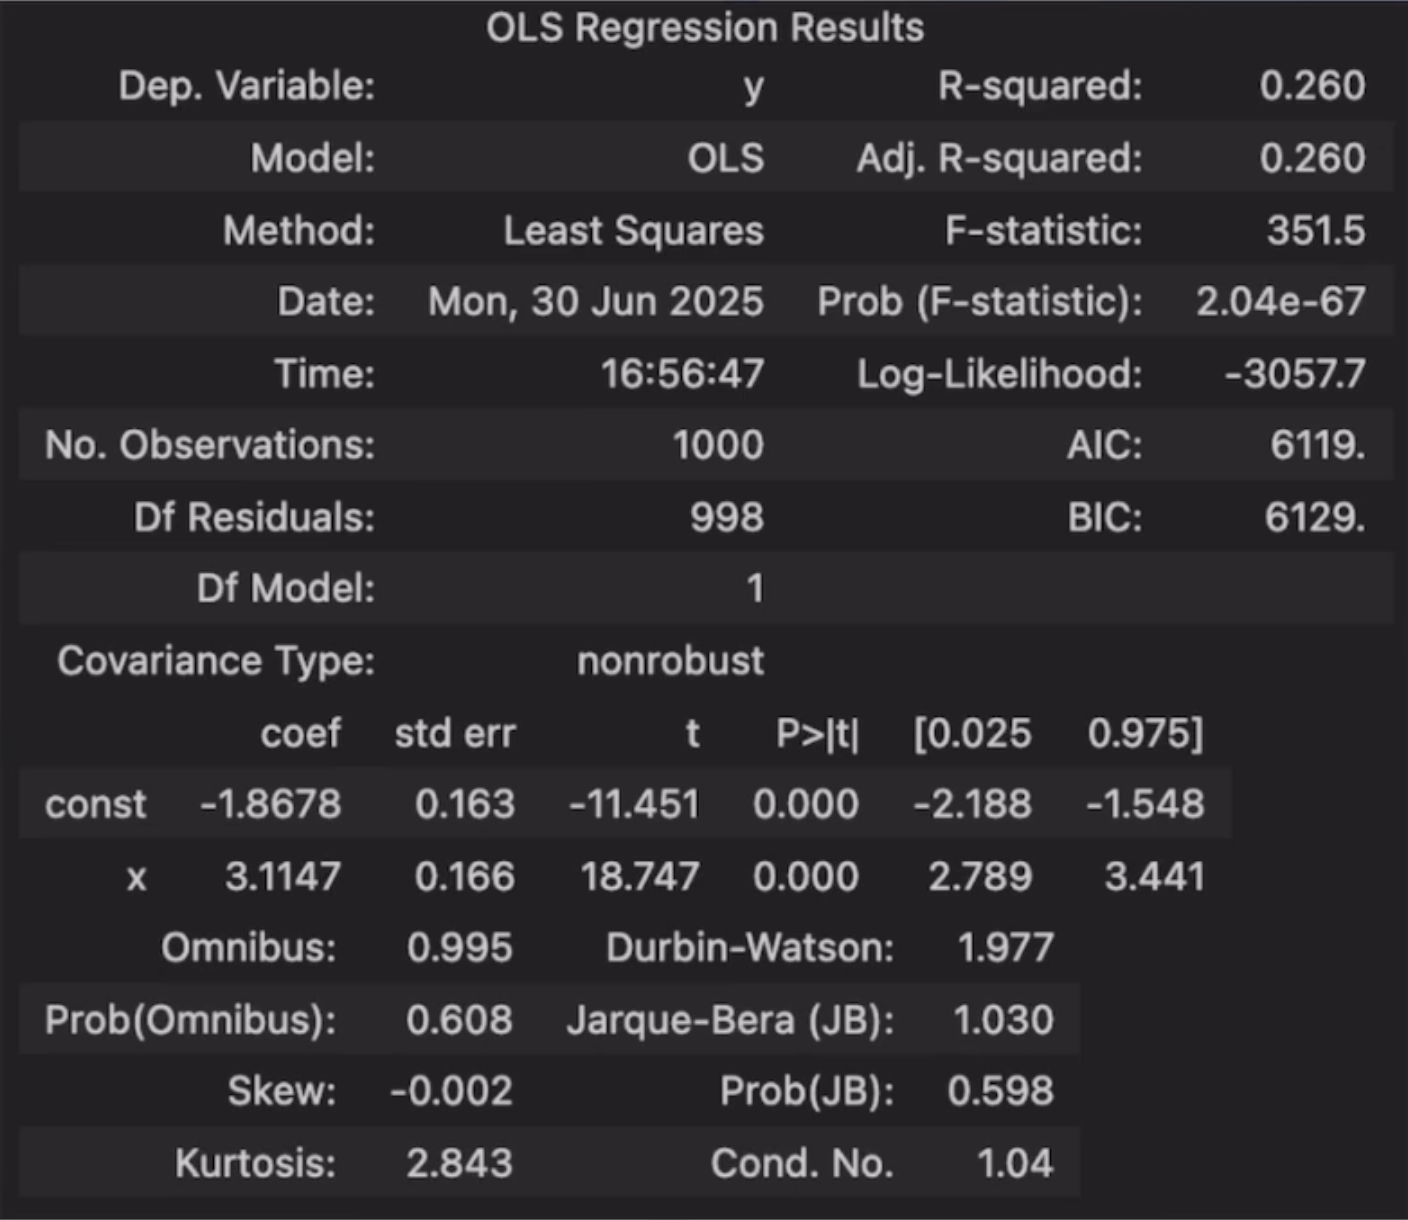
\includegraphics[width=0.5\linewidth]{figs/statsmodels_results.png}
    \caption{Result sample generated by the "statsmodels" package.}
    \label{fig:LRM:statsmodels_results}
\end{figure}

\section{Introduction}

Given \textit{predictors} (\textit{features}) $X^{(1)}, X^{(2)}, \dots, X^{(p-1)}$, $p \geq 2$ and the corresponding \textit{outcome} (\textit{target}) $Y$, the goal of linear regression models is finding linear relationships between the outcomes and all predictors
\begin{align}
    Y = \beta_0 + \beta_1 X^{(1)} + \dots + \beta_{p-1} X^{(p-1)} +\varepsilon,
\end{align}
where $\varepsilon$ is a random noise. In practice, we usually have some observed data points $\{x_i^{(1)}, x_i^{(2)},\dots, x_i^{(p-1)}; y_i\}_{i=1}^{n}$ that can be used to estimate the model, i.e., those unknown regression coefficients, namely $\beta_0,\beta_1,\dots,\beta_{p-1}$, we denote the estimated coefficients as $\hat{\beta}_0,\hat{\beta}_1,\dots,\hat{\beta}_{p-1}$ correspondingly\footnote{They are random variables}. When a new data point (whose outcome is missing) is given, we can let the model process the predictors and thus generate the prediction of this missing outcome. 

The joint distribution of $X^{(1)}, X^{(2)},\dots, X^{(p-1)}, Y$ is extremely complicated in real world, especially when $p$ is large. Therefore, we focus on modeling the conditional statistical properties instead. To be specific, we assume that \ul{the conditional expectation of $Y$ given $X^{(j)} = x^{(j)}$, $1\leq j\leq p-1$ is linear}, that is
\begin{align}
    \mathbb{E}\big[Y | X^{(j)} = x^{(j)}, 1\leq j\leq p-1\big]
    =
    \beta_0 + \sum_{j=1}^{p-1} \beta_jx^{(j)}.
\end{align}
Which means that, for each data point, we have
\begin{align}
    \mathbb{E}\big[Y | X_i^{(j)} = x_i^{(j)}, 1\leq j\leq p-1\big]
    =
    \beta_0 + \sum_{j=1}^{p-1} \beta_jx_i^{(j)}.
\end{align}
We also assume that \ul{$\{Y_i\}_{i=1}^{N}$ are conditional independent}.

\textcolor{red}{For simplicity, we omit the conditional expectation notation in the following discussions. Nevertheless, it is important to keep in mind that all expectations are taken conditionally.}

To fully determine the conditional distribution of $Y$, we also need to specify the conditional distribution of the random noise $\varepsilon$. In these notes, we use \ul{normal distributions with common variance $\sigma^2$} to model $\varepsilon$. Thus, the conditional distribution of $Y_i$ is 
\begin{align}
    \label{eqn:LRM-intro:Y-conditional-distro}
    Y\bigg|\Big\{ X_i^{(j)} = x_i^{(j)}\Big\}_{j=1}^{p-1}
    \sim
    \mathcal{N}
    \left(
    \beta_0 + \sum_{j=1}^{p-1} \beta_jx_i^{(j)}, \sigma^2
    \right).
\end{align}
As previously explained, we may omit the conditional notation in Eq.~(\ref{eqn:LRM-intro:Y-conditional-distro}) for simplicity. The expression can then be written as follows
\begin{align}
    \label{eqn:LRM-intro:Y-simplified-distro}
    Y
    \sim
    \mathcal{N}
    \left(
    \beta_0 + \sum_{j=1}^{p-1} \beta_jx_i^{(j)}, \sigma^2
    \right).
\end{align}
However, we emphasize that Eq.~(\ref{eqn:LRM-intro:Y-simplified-distro}), along with all results derived from it, should be understood as conditional statements.

Additionally, we emphasize that \ul{the variance $\sigma^2$ of the error term $\varepsilon$ is assumed to be a constant across all inputs $\{x_i^{(j)}\}_{j=1}^n$}, a property known as \textit{homoscedasticity}. In contrast, if the variance depends on the inputs $\{x_i^{(j)}\}_{j=1}^n$, the model is said to exhibit \textit{heteroscedasticity}.

\section{Simple Linear Regression}

When $p=2$, the linear regression model becomes $Y = \beta_0 + \beta_1 X + \varepsilon$, which is called \textit{simple linear regression model}.

\subsection{Fitting the Model}

\theorem The regression coefficients of a simple linear regression model are given by
\begin{align}
    \hat{\beta}_1 
    = 
    \frac{\sum_{i=1}^{n}(Y_i-\bar{Y})(x_i - \bar{x})}{\sum_{i=1}^{n}(x_i - \bar{x})^2}, 
    \quad \text{ and }
    \hat{\beta}_0
    = \bar{Y} - \beta_1\bar{x},
    \label{eqn:SLR:regression-coefficients}
\end{align}
where 
\begin{align}
    \bar{Y} = \frac{1}{n}\sum_{i=1}^{n}Y_i.
\end{align}

\noindent \textbf{Notation Remark}: We will use $\hat{\xi}$ as our estimated $\xi$, it can be a number (without randomness) or a random variable (with randomness) depending the context.
\begin{proof}
Our best estimates for $\beta_0$ and $\beta_1$ should minimize the error between the observed responses and the predicted values. One reasonable choice of the error is the mean square error (MSE)\footnote{We briefly note that this is also referred to as the $L_2$ error. Other choices, such as the $L_1$ error, are also possible.}
\begin{align*}
    F(\beta_0,\beta_1) = \frac{1}{n} \sum_{i=1}^n\left[Y_i - (\beta_0 + \beta_1 x_i)\right]^2,
\end{align*}
and we have the following equation
\begin{align*}
    \hat{\beta}_0,\hat{\beta}_1 = \argmin_{\beta_0,\beta_1} F(\beta_0,\beta_1).
\end{align*}
The minimum condition gives the equations for $\hat{\beta}_0,\hat{\beta}_1$
\begin{numcases}{}
    \label{eqn:SLR:dF_db0}
    \pdv{F}{\beta_0}\bigg|_{\hat\beta_0} = 0, \\
    \pdv{F}{\beta_1}\bigg|_{\hat\beta_1} = 0.
    \label{eqn:SLR:dF_db1}
\end{numcases}
Eq.~(\ref{eqn:SLR:dF_db0}) gives 
\begin{align}
    \label{eqn:SLR:dF_db0-expand}
    \frac{-2}{n} \sum_{i=1}^n\left[Y_i - (\hat\beta_0 + \hat\beta_1 x_i)\right] &= 0, \\
    \sum_{i=1}^n (\hat\beta_0 + \hat\beta_1 x_i) &= \sum_{i=1}^nY_i,\notag \\
    n \hat\beta_0 + \hat\beta_1 \sum_{i=1}^n x_i &= \sum_{i=1}^nY_i,\notag \\
    \hat\beta_0 &= \bar{Y} - \hat\beta_1 \bar{x}.\notag
\end{align}
We obtained the expression for $\hat\beta_0$ in the theorem. We proceed our calculation with Eq.~(\ref{eqn:SLR:dF_db1}), it gives 
\begin{align}
    \label{eqn:SLR:dF_db1-expand}
    \frac{-2}{n} \sum_{i=1}^n\left[Y_i - (\hat\beta_0 + \hat\beta_1 x_i)\right]x_i &= 0,\\
    \sum_{i=1}^n (\hat\beta_0 + \hat\beta_1 x_i)x_i &= \sum_{i=1}^nY_i x_i\notag,
\end{align}
Inserting the result for $\hat\beta_0$, yields
\begin{align*}
    (\bar{Y} - \hat\beta_1 \bar{x}) \sum_{i=1}^n x_i + \hat\beta_1  \sum_{i=1}^n x_i^2 &= \sum_{i=1}^nY_i x_i,\\
    \hat\beta_1 ( \sum_{i=1}^n x_i^2 - \bar{x} \sum_{i=1}^n x_i) &= \sum_{i=1}^nY_i x_i - \bar{Y} \sum_{i=1}^n x_i,\\
    \hat\beta_1 ( \sum_{i=1}^n x_i^2 - \bar{x} \sum_{i=1}^n x_i) &= \sum_{i=1}^nY_i x_i - \sum_{i=1}^n Y_i  \bar{x},\\
    \hat\beta_1 \sum_{i=1}^n (x_i - \bar{x}) x_i &= \sum_{i=1}^n(x_i - \bar{x})Y_i,\\
    \hat\beta_1 \sum_{i=1}^n (x_i - \bar{x}) (x_i - \bar{x}) &= \sum_{i=1}^n(x_i - \bar{x})(Y_i - \bar{Y}),\\
    \hat\beta_1 &= \frac{\sum_{i=1}^n(x_i - \bar{x})(Y_i - \bar{Y})}{\sum_{i=1}^n (x_i - \bar{x})^2}.
\end{align*}
Note that, in the calculation, we used the observation that
\begin{align*}
    \sum_{i=1}^n (x_i - \bar{x}) \xi_i &= \sum_{i=1}^n (x_i - \bar{x}) \xi_i - \bar{\xi}\sum_{i=1}^n (x_i - \bar{x})\\
    &= - \sum_{i=1}^n (x_i - \bar{x}) (\bar{\xi}-\xi_i),
\end{align*}
since $\sum_{i=1}^n (x_i - \bar{x}) = 0$. This concludes our proof.
\end{proof}

\corollary The regression line must pass through the point $(\bar{x}, \bar{Y})$.\\
\begin{proof}
This is a simple observation from the regression coefficient $\hat{\beta}_0 = \bar{Y} - \hat{\beta}_{1} \bar{x}$ $\Rightarrow$ $\bar{Y} = \hat{\beta}_0 + \hat{\beta}_{1} \bar{x}$.
\end{proof} 

Suppose that the observed values of $\mathbf{Y} = \{Y_i\}_{i=1}^n$ are $\mathbf{y} = \{y_i\}_{i=1}^n$. With the numbers $\mathbf{y} = \{y_i\}_{i=1}^n$, we can calculate the \textit{fitted values}
\begin{align}
    \hat{y}_i = \hat{\beta}_0 + \hat{\beta}_1 x_i,
\end{align}
and residuals
\begin{align}
    e_i = y_i - \hat{y}_i = y_i - (\hat{\beta}_0 + \hat{\beta}_1 x_i)
\end{align}

\noindent \textbf{Notation Remark}: We will use boldface symbols like $\mathbf{A},\dots ,\mathbf{Z},\boldsymbol{\alpha},\dots,\boldsymbol{\omega}$ to represent vectors and matrices.

\theorem Residuals always satisfy 
\begin{align}
    \begin{cases}
    \sum_{i=1}^{n} e_i = 0,\\
    \sum_{i=1}^{n} x_i e_i = 0.
    \end{cases}
\end{align}
\begin{proof}
This is a simple corollary from Eq.~(\ref{eqn:SLR:dF_db0-expand}) and (\ref{eqn:SLR:dF_db1-expand}).
\end{proof}

The simple linear regression model can be trained by maximum likelihood estimators (MLE) as well.

\theorem Define $\mathbf{x} = \{x_i\}_{i=1}^n$, then the likelihood function $\mathcal{L}_n$ evaluated at $\mathbf{y}$ is 
\begin{align}
    \mathcal{L}_n(\mathbf{y}|\mathbf{x},\beta_0,\beta_1,\sigma^2) = 
    \frac{1}{(2\pi\sigma^2)^{n/2}}
    \exp\left[
    -\frac{1}{2\sigma^2} \sum_{i=1}^n (y_i - \beta_0 -\beta_1 x_i)^2
    \right].
\end{align}
The MLE of the regression coefficients are given in Eq.~(\ref{eqn:SLR:regression-coefficients}), while the MLE of $\sigma^2$ is given by
\begin{align}
    \hat{\sigma}^2 = \frac{1}{n}\sum_{i=1}^n (Y_i - \hat\beta_0 -\hat\beta_1 x_i)^2 = \frac{1}{n}S^2,
\end{align}
where $S^2$ is the sum of squared errors under the best estimation for $\beta_0$ and $\beta_1$, that is, $S^2 = F(\hat\beta_0,\hat\beta_1)$.

\noindent \textbf{Remark}: The estimated $\hat{\sigma}^2$ is biased, in fact,
\begin{align*}
    \frac{n\hat{\sigma}^2}{\sigma^2} \sim \chi^2(n-2).
\end{align*}
We will show this later.
\begin{proof}
Suppose that we are given a sample $y_i$ from $Y_i$, the possibility of observing this particular sample is, i.e., its' likelihood function $\mathcal{L}$ is 
\begin{align}
    \mathcal{L}_i(y_i|x_i,\beta_0,\beta_1,\sigma^2) = 
\frac{1}{\sigma\sqrt{2\pi}}
\exp\left[
-\frac{1}{2\sigma^2}(y_i - \beta_0 -\beta_1 x_i)^2
\right].
\end{align}
Since $\{Y_i\}_{i=1}^{N}$ are conditional independent, if we are giving a set of samples $\mathbf{y}=\{y_i\}_{i=1}^N$, we can simply multiply the likelihood function of single data point to get the likelihood function for $\mathbf{y}$: 
\begin{align*}
    \mathcal{L}_n(\mathbf{y}|\mathbf{x},\beta_0,\beta_1,\sigma^2) = 
    \frac{1}{(2\pi\sigma^2)^{n/2}}
    \exp\left[
    -\frac{1}{2\sigma^2} \sum_{i=1}^n (y_i - \beta_0 -\beta_1 x_i)^2
    \right].
\end{align*}
When training the model, we aim to maximize the likelihood function $\mathcal{L}_n$. In other words, we seek the coefficients $\hat\beta_0$ and $\hat\beta_1$ that maximize the likelihood of observing the given dataset. Mathematically, its optimization is equivalent to minimizing the MSE\footnote{In the following equation, $y_i$ is replaced to $Y_i$, since the argument holds for any dataset. It is similar to the argument we make later in the text for $\hat\sigma^2$.}, $nF(\beta_0,\beta_1) = \sum_{i=1}^n\left[Y_i - (\beta_0 + \beta_1 x_i)\right]^2$. As a result, both approaches yield the same estimates for $\beta_0$ and $\beta_1$ in the linear regression model, with their expressions given in Eq.~(\ref{eqn:SLR:regression-coefficients}).

Additionally, the best estimate of $\sigma^2$ should maximize $\mathcal{L}_n$ (the probability) as well, we have
\begin{align*}
    \pdv{\mathcal{L}_n}{\sigma^2} &= 0,\\
    \frac{-n/2}{(2\pi)^{n/2}} \frac{1}{(\sigma^2)^{n/2+1}}\exp\left[-\frac{F(\beta_0,\beta_1|\mathbf{y})}{2\sigma^2}\right] + \frac{-1}{(2\pi)^{n/2}} \frac{1}{(\sigma^2)^{n/2}}\exp\left[-\frac{F(\beta_0,\beta_1|\mathbf{y})}{2\sigma^2}\right] \left(\frac{F(\beta_0,\beta_1|\mathbf{y})}{2}\frac{1}{(\sigma^2)^2}\right) &= 0,\\
    -n + \frac{F(\beta_0,\beta_1|\mathbf{y})}{\sigma^2} &= 0,\\
    \sigma^2 &= \frac{F(\beta_0,\beta_1|\mathbf{y})}{n}.
\end{align*}
Since this analysis holds for any dataset, we can remove the "conditioned on $\mathbf{y}$" in the equations, and get the best estimation for $\sigma^2$ as $\hat\sigma^2 = \frac{1}{n}F(\hat\beta_0,\hat\beta_1) = \frac{1}{n}S^2$.
\end{proof}

\noindent \textbf{Notation Remark}: We will use the notation
\begin{align}
    s_x = \sqrt{\sum_{i=1}^{n}(x_i - \bar{x}_i)^2},
\end{align}
in the following discussions.

\subsubsection{Distributions of the estimators}

\theorem 
\label{thm:SLR:beta_0_1_dist_cov}
The following claims hold for distributions of $\hat{\beta}_0$ and $\hat{\beta}_1$ 
\begin{enumerate}
\item 
\begin{align}
    \hat\beta_0 \sim \mathcal{N}\left(\beta_0,\sigma^2\left(\frac{1}{n} + \frac{\bar{x}^2}{s_x^2}\right)\right).
    \label{eqn:SLR:beta_0_dist}
\end{align}
\item 
\begin{align}
    \hat\beta_1 \sim \mathcal{N}\left(\beta_1,\frac{\sigma^2}{s_x^2}\right).
    \label{eqn:SLR:beta_1_dist}
\end{align}
\item 
\begin{align}
    \cov(\hat{\beta}_0,\hat{\beta}_1) = -\frac{\bar{x}\sigma^2}{s_x^2}.
    \label{eqn:SLR:cov_beta_0_beta_1}
\end{align}
\end{enumerate}

\begin{proof}
Let's start with $\hat{\beta}_1$ in Eq.~(\ref{eqn:SLR:regression-coefficients}), we have
\begin{align*}
    \hat{\beta}_1 &= \frac{\sum_{i=1}^n Y_i (x_i - \bar{x})}{s_x^2},\\
    &= \frac{\sum_{i=1}^n (\beta_0 + \beta_1 x_i + \varepsilon_i) (x_i - \bar{x})}{s_x^2},\\
    &= \frac{\sum_{i=1}^n (\beta_0 + \beta_1 x_i) (x_i - \bar{x})}{s_x^2} + \sum_{i=1}^{n} \frac{(x_i - \bar{x})}{s_x^2}\varepsilon_i,\\
    &\sim \beta_1 \frac{\sum_{i=1}^n x_i (x_i - \bar{x})}{s_x^2} + \sum_{i=1}^{n} \frac{(x_i - \bar{x})}{s_x^2}\mathcal{N}(0,\sigma^2),\\
    &= \beta_1 \frac{\sum_{i=1}^n(x_i - \bar{x})^2}{s_x^2} + \mathcal{N}\left(0,\sum_{i = 1}^{n}\frac{(x_i - \bar{x})^2}{(s_x^2)^2}\sigma^2\right),\quad (\varepsilon_i\text{ are independent})\\
    &= \beta_1 + \mathcal{N}\left(0,\frac{\sigma^2}{s_x^2}\right),\\
    &= \mathcal{N}\left(\beta_1, \frac{\sigma^2}{s_x^2}\right).\\
\end{align*}
We obtain the result in Eq.~(\ref{eqn:SLR:beta_1_dist}). Note that, in the calculation, we repeatedly use the property that $\sum_i c(x_i-\bar{x}) = 0$, where $c$ is a constant.

Next, let's calculate the distribution of $\hat{\beta}_0$, starting from Eq.~(\ref{eqn:SLR:regression-coefficients}),
\begin{align*}
    \hat{\beta}_0 &= \bar{Y} - \hat\beta_1 \bar{x},\\
    &= \bar{Y} - \frac{\sum_{i=1}^n Y_i (x_i - \bar{x})}{s_x^2} \bar{x},\\
    &= \frac{\sum_{i=1}^n \left[Y_i \frac{s_x^2}{n} - Y_i \bar{x}(x_i - \bar{x})\right]}{s_x^2},\\
    &= \frac{1}{s_x^2}\sum_{i=1}^n \left[ \frac{s_x^2}{n} - \bar{x}(x_i - \bar{x})\right](\beta_0 +\beta_1  x_i +\varepsilon_i),\\
    &=  \frac{1}{s_x^2}
    \left\{
    \sum_{i=1}^n \left[ \frac{s_x^2}{n} - \bar{x}(x_i - \bar{x})\right](\beta_0 +\beta_1  x_i) + 
    \sum_{i=1}^n \left[ \frac{s_x^2}{n} - \bar{x}(x_i - \bar{x})\right] \varepsilon_i
    \right\},\\
    &\sim \frac{1}{s_x^2}
    \left\{
    \beta_0 s_x^2 + \beta_1 \bar{x} s_x^2 - 
    \beta_1 \bar{x}  \sum_{i=1}^n (x_i - \bar{x})( x_i) + 
    \sum_{i=1}^n \left[ \frac{s_x^2}{n} - \bar{x}(x_i - \bar{x})\right] \mathcal{N}(0,\sigma^2)
    \right\},\\
    &= \beta_0 + 
    \sum_{i=1}^n \left[ \frac{1}{n} - \frac{\bar{x}(x_i - \bar{x})}{s_x^2}\right] \mathcal{N}(0,\sigma^2),\\
    &= \beta_0 + 
     \mathcal{N}\left(0,\sigma^2 \sum_{i=1}^n \left[ \frac{1}{n} - \frac{\bar{x}(x_i - \bar{x})}{s_x^2}\right]^2\right),\quad (\varepsilon_i\text{ are independent})\\
    &= \mathcal{N}\left(\beta_0,\sigma^2 \left(\frac{1}{n} + \frac{\bar{x}^2}{s_x^2}\right) \right),
\end{align*}
where the sum of the variances in the final step is straightforward to compute,
\begin{align*}
    \sum_{i=1}^n \left[ \frac{1}{n} - \frac{\bar{x}(x_i - \bar{x})}{s_x^2}\right]^2
    &= \sum_{i=1}^n \left[ \frac{1}{n^2} + \frac{\bar{x}^2(x_i - \bar{x})^2}{(s_x^2)^2} - \frac{2}{n}\frac{\bar{x}(x_i - \bar{x})}{s_x^2}\right],\\
    &= \frac{1}{n} + \frac{\bar{x}^2}{s_x^2}. 
\end{align*}
We have to emphasize that we can not use the distribution of $\hat{\beta}_1$ we just calculated, since it is correlated with $Y_i$ and we don't know the covariance yet.

To complete the proof of the theorem, it remains to show the covariance, for which we have
\begin{align*}
    \cov(\hat\beta_0,\hat\beta_1) &= \cov(\bar{Y} - \hat{\beta_1}\bar{x},\hat\beta_1),\\
    &= \cov(\bar{Y},\hat\beta_1) - 
    \bar{x} \varr(\hat{\beta_1}),\\
    &= \cov
    \left(
    \sum_{i=1}^{n}\frac{1}{n}Y_i, 
    \frac{\sum_{j=1}^n Y_j (x_j - \bar{x})}{s_x^2}
    \right) - 
    \bar{x} \varr(\hat{\beta_1}),\\
    &= \sum_{i=1}^n\sum_{j=1}^n\frac{1}{n} \frac{(x_j - \bar{x})}{s_x^2} \cov(Y_i, Y_j) - 
    \bar{x} \frac{\sigma^2}{s_x^2},\\
    &= \sum_{i=1}^n\sum_{j=1}^n\frac{1}{n} \frac{(x_j - \bar{x})}{s_x^2} \sigma^2 \delta_{ij} - 
    \frac{\bar{x} \sigma^2}{s_x^2},\\
    &= - \frac{\bar{x} \sigma^2}{s_x^2}.
\end{align*}
So far we have concluded our proof.
\end{proof}

\problem Write a program to verify these claims.

\problem Let $H = c_0 \hat\beta_0 + c_1 \hat\beta_1$ be a linear combination of $\hat{\beta_0}$ and $\hat{\beta_1}$ show that the variance of $H$ is given by
\begin{align*}
    \varr(H) = \sigma^2 \left[ \frac{c_0^2}{n} + \frac{(c_0\bar{x} - c_1)^2}{s_x^2}\right].
\end{align*}
\begin{proof}
We have
\begin{align*}
    \varr(H) &= \varr(c_0 \hat\beta_0 + c_1 \hat\beta_1),\\
    &= c_0^2 \varr(\hat\beta_0)  + c_1^2 \varr(\hat\beta_1) + 2c_0c_1 \cov(\hat\beta_0, \hat\beta_1),\\
    &= 
    c_0^2 
    \sigma^2 \left(\frac{1}{n} + \frac{\bar{x}^2}{s_x^2}\right) + c_1^2 
    \frac{\sigma^2}{s_x^2} - 
    2c_0c_1 
    \frac{\bar{x} \sigma^2}{s_x^2},\\
    &= \sigma^2 \left[
    \frac{c_0^2 }{n} + 
    \frac{(c_0\bar{x} - c_1)^2}{s_x^2}
    \right].\\
\end{align*}
\end{proof}

Now suppose that a linear regression model has been trained through data points $\{x_i, y_i\}_{i=1}^n$. When a test data point $x$ is coming, we can the use the model to predict the outcome $Y$ for $x$.

By the setting of  simple linear regression models, $Y$ is a random variable following the normal distribution with mean $\beta_0 + \beta_1 x$ and variance $\sigma^2$. It is natural to use $\hat{Y} = \hat{\beta}_0 + \hat{\beta}_1 x$ as the prediction of $Y$, which will surely introduce errors. We can measure this error through the mean squared error.

\theorem The MSE of $Y$ is given by
\begin{align}
    \mathbb{E}\Big[\big(Y - \hat{Y}\big)^2\Big] = \sigma^2
    \left[
    1 + \frac{1}{n} +\frac{(x - \bar{x})^2}{s_x^2}
    \right].
\end{align}
\noindent \textbf{Remark}: The MSE gets larger as $x$ moves away from the observed training data. Is this correct intuitively?
\begin{proof}
The expectation we want to show can be written as
\begin{align*}
    \mathbb{E}\Big[\big(Y - \hat{Y}\big)^2\Big] &= \mathbb{E}\big[Y^2 + \hat{Y}^2 - 2 Y \hat{Y} \big],\\
    &= \mathbb{E}\big[Y^2\big] + \mathbb{E}\big[\hat{Y}^2\big] - 2 \mathbb{E}\big[Y \hat{Y} \big].
\end{align*}
For each term on the RHS, we have
\begin{align*}
    \mathbb{E}\big[Y^2\big] &= \varr(Y) + \mathbb{E}[Y]^2,\\
    &= \sigma^2 + (\beta_0 + \beta_1 x)^2,\\
    \mathbb{E}\big[\hat{Y}^2\big] &=  \varr(\hat{Y}) + \mathbb{E}[\hat{Y}]^2,\\
    &= \varr(\hat{\beta}_0 + \hat{\beta}_1 x) + (\beta_0 + \beta_1 x)^2,\\
    &= \sigma^2\left(\frac{1}{n} + \frac{(\bar{x} - x)^2}{s_x^2}\right) + (\beta_0 + \beta_1 x)^2,\\
    \mathbb{E}\big[Y \hat{Y} \big] &= \mathbb{E}\big[Y (\hat{\beta}_0 + \hat{\beta}_1 x) \big],\\
    &= \mathbb{E}\big[Y \hat{\beta}_0\big] + x \mathbb{E}\big[ Y \hat{\beta}_1 \big],\\
    &= \mathbb{E}[Y] \mathbb{E}\big[\hat{\beta}_0\big] + x \mathbb{E}[Y] \mathbb{E}\big[\hat{\beta}_1 \big],\quad (Y\text{ and }\hat\beta_{0,1}\text{ are independent by definition})\\
    &= (\beta_0 + \beta_1 x)^2.
\end{align*}
Put them together, we find
\begin{align*}
    \mathbb{E}\Big[\big(Y - \hat{Y}\big)^2\Big] &= \sigma^2 + (\beta_0 + \beta_1 x)^2 + \sigma^2\left(\frac{1}{n} + \frac{(\bar{x} - x)^2}{s_x^2}\right) + (\beta_0 + \beta_1 x)^2 - 2 (\beta_0 + \beta_1 x)^2,\\
    &= \sigma^2
    \left[
    1 + \frac{1}{n} +\frac{(x - \bar{x})^2}{s_x^2}
    \right].
\end{align*}
That concludes our calculation.
\end{proof}

In order to obtain the joint distribution of $\hat{\beta}_0, \hat{\beta}_1$ and $\hat{\sigma}^2$, we need the following lemmas.

\lemma 
\label{lam:SLR:bivariate-tf}
Random variables $(P_1, P_2)$ follow \textit{bivariate normal distribution}. Define $(Q_1, Q_2)$ as linear combinations of constant $1$, $P_1$ and $P_2$
\begin{align}
    \begin{pmatrix}
        Q_1\\Q_2
    \end{pmatrix}
    =
    \begin{pmatrix}
        a_{11} & a_{12} \\
        a_{21} & a_{22} 
    \end{pmatrix}
    \begin{pmatrix}
        P_1\\P_2
    \end{pmatrix} 
    + 
    \begin{pmatrix}
        b_1\\b_2
    \end{pmatrix},
    \label{eqn:SLR:bivariate-tf}
\end{align}
where 
$\begin{vmatrix}
a_{11} & a_{12}\\
a_{21} & a_{22} 
\end{vmatrix}
\neq 0$.
Then $(Q_1, Q_2)$ also follow bivariate normal distribution.

\begin{proof}
We can write Eq.~(\ref{eqn:SLR:bivariate-tf}) in matrix form for simplicity, i,e., 
\begin{align*}
    \mathbf{Q} = \mathbf{A} \mathbf{P} + \mathbf{b}.
\end{align*}
Let $\boldsymbol{\lambda} \in \mathbb{R}^2 \setminus \{\mathbf{0}\}$, we have 
\begin{align*}
    \boldsymbol{\lambda}^\T\mathbf{Q} &= \boldsymbol{\lambda}^\T(\mathbf{A} \mathbf{P} + \mathbf{b}), \\
    &= (\boldsymbol{\lambda}^\T\mathbf{A}) \mathbf{P} + \boldsymbol{\lambda}^\T\mathbf{b}.
\end{align*}
When $\det \mathbf{A} \neq 0$, we have $\boldsymbol{\lambda}^\T\mathbf{A} \in \mathbb{R}^2 \setminus \{\mathbf{0}\}$. 
Since $\mathbf{P}$ is bivariate normal, it follows by definition that $(\boldsymbol{\lambda}^\T\mathbf{A}) \mathbf{P}$ is normal distributed. 
Therefore $\boldsymbol{\lambda}^\T\mathbf{Q} = (\boldsymbol{\lambda}^\T\mathbf{A}) \mathbf{P} + \boldsymbol{\lambda}^\T\mathbf{b}$ is also normally distributed.
Hence, $\mathbf{Q}$ follows a bivariate normal distribution.
\end{proof}

\lemma
\label{lma:SLR:multi-normal-tf}
Suppose that $\mathbf{P} = \{P_i\}_{i=1}^n$ are i.i.d. and each has distribution $\mathcal{N}(0,1)$. Let $\mathbf{A} \in \mathrm{O}(n)$ be an orthogonal matrix and $\mathbf{Q} = \mathbf{A} \mathbf{P}$, then $\mathbf{Q} = \{Q_i\}_{i=1}^n$ are i.i.d. and each has distribution $\mathcal{N}(0,1)$ as well. additionally, we have $\sum_{i=1}^{n}P_i^2 = \sum_{i=1}^{n}Q_i^2$.
\begin{proof}
The joint probability density function (PDF) of $\mathbf{P}$ is 
\begin{align*}
    f_{\mathbf{P}}(\mathbf{p}) = \prod_{i=1}^n\frac{1}{\sqrt{2\pi}}\exp(-\frac{p_i^2}{2}) = \frac{1}{({2\pi})^{n/2}}\exp(-\frac{\sum_{i=1}^np_i^2}{2}) = \frac{1}{({2\pi})^{n/2}}\exp(-\frac{\mathbf{p}^\T\mathbf{p}}{2}).
\end{align*}
Since the variable transformation should conserve the probability in an infinitesimal volume in $\mathbb{R}^{n}$, we have
\begin{align*}
    g_{\mathbf{Q}}(\mathbf{q})\dd\mathbf{q} &= f_{\mathbf{P}}(\mathbf{p})\dd\mathbf{p},\\
    g_{\mathbf{Q}}(\mathbf{q}) &= f_{\mathbf{P}}(\mathbf{p}) \left|\pdv{\mathbf{p}}{\mathbf{q}}\right|,\\
    &= f_{\mathbf{P}}(\mathbf{A}^{-1}\mathbf{q}) |\det(A^{-1})|.
\end{align*}
Noting that $\mathbf{A}^{-1} = \mathbf{A}^\T$, the PDF of $\mathbf{Q}$ is
\begin{align*}
    g_\mathbf{Q}(\mathbf{q}) &= f_{\mathbf{P}}(\mathbf{A}^\T\mathbf{q}),\\
    &= \frac{1}{({2\pi})^{n/2}}\exp(-\frac{\mathbf{q}^\T\mathbf{A}^\T\mathbf{A}\mathbf{q}}{2}),\\
    &= \frac{1}{({2\pi})^{n/2}}\exp(-\frac{\mathbf{q}^\T\mathbf{q}}{2}).
\end{align*}
Therefore, we find that $\mathbf{Q} = \{Q_i\}_{i=1}^n$ are i.i.d. and each has distribution $\mathcal{N}(0,1)$.

Note that the squared sum property follows directly from the fact that $\mathbf{A}\in\mathrm{O}(n)$,
\begin{align*}
    \sum_{i=1}^{n}Q_i^2 = \mathbf{Q}^\T \mathbf{Q} = \mathbf{P}^\T \mathbf{A}^\T \mathbf{A} \mathbf{P} = \mathbf{P}^\T \mathbf{P} = \sum_{i=1}^{n}P_i^2.
\end{align*}
\end{proof}

Back to our discussion in linear regression, we have the following theorem.

\theorem 
\label{thm:SLR:multi-var-tf}
Let $\mathbf{A} \in \mathrm{O}(n)$ be an orthogonal matrix and $\mathbf{Z} = \mathbf{A} \mathbf{Y}$, where $\mathbf{Y} = \{Y_i\}_{i=1}^n$ are independent normal distributions with mean $\boldsymbol{\mu}$ and  covariance matrix $\sigma^2\mathbf{I}$. Then $\mathbf{Z} = \{Z_i\}_{i=1}^n$ are independent normal distributions with mean $\boldsymbol{\mu}' = \mathbf{A}\boldsymbol{\mu}$ and covariance matrix $\sigma^2\mathbf{I}$.
\begin{proof}
Let $\mathbf{R} = \frac{1}{\sigma}(\mathbf{Y} - \boldsymbol{\mu})$, then $\mathbf{R}$ follows i.i.d. standard normal distribution. From Lemma~\ref{lma:SLR:multi-normal-tf}, we know that $\mathbf{S} = \mathbf{A}\mathbf{R}$ follows i.i.d. standard normal distribution. On the other hand, we have 
\begin{align*}
    \mathbf{Z} = \mathbf{A} \mathbf{Y} = \mathbf{A} (\sigma\mathbf{R} + \boldsymbol{\mu}) = \sigma \mathbf{S} + \mathbf{A}\boldsymbol{\mu}.
\end{align*}
Thus, it is clear that $\mathbf{Z} = \{Z_i\}_{i=1}^n$ satisfies nulti-normal distributions $\mathcal{N}(\mathbf{A}\boldsymbol{\mu},\sigma^2\mathbf{I})$.
\end{proof}

\theorem For a simple linear regression model, we have 
\begin{enumerate}
\item $(\hat{\beta}_0, \hat{\beta}_1)$ follows bivariate normal distribution
\begin{align}
    \begin{pmatrix}
        \hat{\beta}_0\\ \hat{\beta}_1
    \end{pmatrix}
    \sim
    \mathcal{N}\left(
    \begin{pmatrix}
        \beta_0\\\beta_1
    \end{pmatrix},\sigma^2
    \begin{pmatrix}
        \frac{1}{n} + \frac{\bar{x}^2}{s_x^2} & -\frac{\bar{x}}{s_x^2}\\
        -\frac{\bar{x}}{s_x^2} & \frac{1}{s_x^2}
    \end{pmatrix},
    \right)
\end{align}
and the marginal distributions are given in Eq.~(\ref{eqn:SLR:beta_0_dist}) and (\ref{eqn:SLR:beta_1_dist}).
\item $\hat{\sigma}^2$ is independent of $(\hat{\beta}_0, \hat{\beta}_1)$ and 
\begin{align}
    \frac{n\hat{\sigma}^2}{\sigma^2} \sim \chi^2(n-2).
\end{align}
\end{enumerate}

\begin{proof}
\begin{enumerate}
\item Following theorem~\ref{thm:SLR:beta_0_1_dist_cov}, we only need to show that $(\hat{\beta}_0, \hat{\beta}_1)$ follows bivariate normal distribution to finish the proof\footnote{Note that \href{https://statproofbook.github.io/P/norm-margjoint.html}{marginally normal does not imply jointly normal}!}. 

Let's construct the following $\mathbf{A} \in \mathrm{O}(n)$,
\begin{align}
    \label{eqn:SLR:A-mat}
    \mathbf{A} = 
    \begin{pmatrix}
        \frac{1}{\sqrt{n}} & \frac{1}{\sqrt{n}} & \cdots & \frac{1}{\sqrt{n}}\\
        \frac{x_1-\bar{x}}{s_x} & \frac{x_2-\bar{x}}{s_x} & \cdots & \frac{x_n-\bar{x}}{s_x}\\
        \vdots & \vdots & \vdots & \vdots
    \end{pmatrix},
\end{align}
and denote the first row as $\mathbf{a}_{1}$, the second row as $\mathbf{a}_{2}$\footnote{We define $\mathbf{a}_{1,2}$ as column vectors to make the notation clear, that a vector $\mathbf{v}$ is always a column vector.}. It is simple to verify that $\mathbf{a}_{1}$ and $\mathbf{a}_{2}$ are orthogonal and normalized to $1$:
\begin{align*}
    \|\mathbf{a}_{1}\|_2^2 &= \sum_{i = 1}^{n}\frac{1}{n} = 1,\\
    \|\mathbf{a}_{2}\|_2^2 &= \sum_{i = 1}^{n}\frac{(x_i-\bar{x})^2}{s_x^2} = 1,\\
    \mathbf{a}_{1}^\T \mathbf{a}_{2} &= \sum_{i=1}^n\frac{x_i-\bar{x}}{\sqrt{n}s_x} = 0.
\end{align*}
The exact form of the rest rows are unimportant to our proof, and we simply note that they can be constructed from the Gram–Schmidt process. 

Let $\mathbf{Z} = \mathbf{A}\mathbf{Y}$, from theorem~\ref{thm:SLR:multi-var-tf}, we know that $\mathbf{Z} = \{Z_i\}_{i=1}^{n}$ are independent normal distributions with the same variance $\sigma^2$. In particular, $Z_1$ and $Z_2$ are independent normal distributions with the same variance $\sigma^2$. Additionally, we have 
\begin{align*}
    Z_1 &= \sum_{i=1}^n a_{1i} Y_{i} = \sqrt{n}\bar{Y} = \sqrt{n}(\hat{\beta}_0 + \hat{\beta}_1\bar{x}) ,\\
    Z_2 &= \sum_{i=1}^n a_{2i} Y_{i} = \sum_{i=1}^n\frac{(x_i-\bar{x})Y_i}{s_x} = s_x\hat{\beta}_1.
\end{align*}
Solving $\hat{\beta}_0$ and $\hat{\beta}_1$ from it, we have
% \begin{align*}
%     \hat\beta_0 &= \frac{1}{\sqrt{n}}Z_1 - \frac{\bar{x}}{s_x} Z_2,\\
%     \hat\beta_1 &= \frac{1}{s_x} Z_2.
% \end{align*}
% That is 
\begin{align}
    \label{eqn:SLR:beta_Z_mat}
    \begin{pmatrix}
        \hat\beta_0 \\ \hat\beta_1
    \end{pmatrix}
    =
    \begin{pmatrix}
        \frac{1}{\sqrt{n}} & - \frac{\bar{x}}{s_x}\\
        0 & \frac{1}{s_x}
    \end{pmatrix}
    \begin{pmatrix}
        Z_1\\Z_2
    \end{pmatrix},
\end{align}
in the matrix from. Clearly 
\begin{align*}
    \begin{vmatrix}
        \frac{1}{\sqrt{n}} & - \frac{\bar{x}}{s_x}\\
        0 & \frac{1}{s_x}
    \end{vmatrix}
    = 
    \frac{1}{\sqrt{n}s_x} \neq 0.
\end{align*}
From lemma~\ref{lam:SLR:bivariate-tf}, we conclude that $(\hat{\beta}_0, \hat{\beta}_1)$ follows bivariate normal distribution. Additionally, during the proof, we observe that $Z_1, Z_2$ have variance $\sigma^2$. By the property of normal distributions, we can get the covariance matrix immediately from Eq.~(\ref{eqn:SLR:beta_Z_mat}).

\item Recall that our estimation for $\hat\sigma^2$ is 
\begin{align*}
    \hat\sigma^2 = \frac{1}{n}S^2 = \frac{1}{n}\sum_{i=1}^n(Y_i - \hat\beta_0 - \hat\beta_1 x_i)^2.
\end{align*}
The approach is to make connection with the $\mathbf{A}$ matrix we defined in Eq.~(\ref{eqn:SLR:A-mat}). By Eq.~(\ref{eqn:SLR:beta_Z_mat}), we have
\begin{align*}
    \hat\sigma^2 &= \frac{1}{n}\sum_{i=1}^n\left[Y_i - \left(\frac{1}{\sqrt{n}}Z_1 - \frac{\bar{x}}{s_x} Z_2\right) - \frac{1}{s_x} Z_2 x_i\right]^2,\\
    &= \frac{1}{n}\sum_{i=1}^n
    \left[
    Y_i - 
    \frac{1}{\sqrt{n}}Z_1 - \frac{x_i - \bar{x}}{s_x} Z_2 
    \right]^2,\\
    &= \frac{1}{n}\sum_{i=1}^n
    \left[
    Y_i - 
    a_{1i}Z_1 - a_{2i} Z_2
    \right]^2,\\
    &= \frac{1}{n}\left\|
    \mathbf{Y} -
    \mathbf{a}_{1} Z_1 -
    \mathbf{a}_{2} Z_2
    \right\|_2^2,\\
    &= 
    \frac{1}{n}\left(
    \mathbf{Y}^\T \mathbf{Y} +
    \mathbf{a}_{1}^\T \mathbf{a}_{1}Z_1^2 +
    \mathbf{a}_{2}^\T \mathbf{a}_{2} Z_2^2 - 
    2 \mathbf{Y}^\T \mathbf{a}_{1} Z_1 - 
    2 \mathbf{Y}^\T \mathbf{a}_{2} Z_2 +
    2 \mathbf{a}_{1}^\T \mathbf{a}_{2} Z_1 Z_2
    \right)
    ,\\
    &= 
    \frac{1}{n}\left(
    \mathbf{Y}^\T \mathbf{Y} +
    Z_1^2 +
    Z_2^2 - 
    2 (\mathbf{a}_{1}^\T \mathbf{Y})^\T Z_1 - 
    2 (\mathbf{a}_{2}^\T \mathbf{Y})^\T Z_2 
    \right)
    ,\quad (\mathbf{A} \in \mathrm{O}(n))\\
    &= 
    \frac{1}{n}\left(
    \mathbf{Y}^\T \mathbf{Y} -
    Z_1^2 -
    Z_2^2 
    \right)
    ,\quad (\mathbf{Z} = \mathbf{A}\mathbf{Y})\\
    &= 
    \frac{1}{n}\left(
    \mathbf{Z}^\T \mathbf{Z} -
    Z_1^2 -
    Z_2^2 
    \right)
    ,\quad \text{(lemma~\ref{lma:SLR:multi-normal-tf})}\\
    &= 
    \frac{1}{n}\sum_{i=3}^{n}Z_i^2,\\
\end{align*}
Next, for the purpose of normalization, we calculate the mean of $Z_i$,
\begin{align*}
    \mathbb{E}[Z_i] &= \mathbb{E}[\mathbf{a}_i^\T \mathbf{Y}],\\
    &= \mathbb{E}[\mathbf{a}_i^\T (\beta_0 + \beta_1 \mathbf{x} + \boldsymbol{\varepsilon})],\\
    &= \mathbb{E}[\mathbf{a}_i^\T (\hat\beta_0 + \hat\beta_1 \mathbf{x} )],\\
    &= \mathbb{E}[\mathbf{a}_i^\T (\mathbf{a}_1 Z_1 + \mathbf{a}_2 Z_2)],\\
    &= 0, \quad \text{ when }i\geq 3.
\end{align*}
Therefore, we have
\begin{align*}
    \frac{n\hat{\sigma}^2}{\sigma^2} = 
    \sum_{i=3}^{n}\left(\frac{Z_i}{\sigma}\right)^2
    \sim \chi^2(n-2).\\
\end{align*}
That concludes our proof.
\end{enumerate}
\end{proof}

\noindent \textbf{Summary} 

In this section, we introduced two methods to train an simple linear regression model: (1) by minimizing the mean squared error, and (2) by maximizing the likelihood function. We show that their results are the same. Additionally, we derived the joint distribution of $\hat{\beta}_0, \hat{\beta}_1$ and $\hat{\sigma}^2$.

\subsection{Statistical Tests}

\section{Multiple Linear Regression}

\subsection{Fitting the Model}

\subsection{Statistical Tests}

\section{Multicolinearity}

\section{$R$-Squared and Adjusted $R$-Squared}

\section{AIC and BIC}

\section{Other Details}

\ifdefined\isSubfile
\else
  % \bibliographystyle{alpha}
  % \bibliography{ref}
  \end{document}
\fi
